\documentclass[aps,
%prl,
twocolumn,
%showpacs,
superscriptaddress,groupedaddress]{revtex4}


\usepackage{amssymb}
\usepackage{amsmath}
\usepackage{float}
\usepackage{graphicx}
\usepackage[caption=false]{subfig}
\usepackage{subfig}
\usepackage{mathrsfs}

\newcommand{\dmcomment}[1]{{\tt #1}}

\begin{document}

\title{Theory of the crossover from lasing to steady state superradiance}
\author{D. A. Tieri}
\affiliation{JILA, University of Colorado, Boulder}
\author{Minghui Xu}
\affiliation{JILA, University of Colorado, Boulder}
\author{J. Cooper}
\affiliation{JILA, University of Colorado, Boulder}
\author{D. Meiser}
\affiliation{Tech-X Corporation, 5621 Arapahoe Avenue,
             Boulder, Colorado 80303, USA.}
\author{M. J. Holland}
\affiliation{JILA, University of Colorado, Boulder}
\date{\today}

\begin{abstract}
  Lasing and steady state superradiance are two phenomena that may
  appear at first glance to be distinct, but in fact should be thought
  of as the two extreme limits of a continuous crossover. In a laser,
  the macroscopic field that stores the phase information is the
  intracavity light field, and the robustness of this phase is what
  leads to the coherence properties of the output light. In contrast,
  in steady-state superradiant systems, the coherence derives from the
  macroscopic collective dipole of a many-atom ensemble. In this
  paper, we develop a quantum theory that connects smoothly between
  these two extreme limits by showing that coherence can be
  simultaneously stored in both atoms and light. The properties of
  systems that lie in the superradiance, lasing, and crossover parameter
  regions are contrasted and compared. We find that a system in the
  crossover region can operate much farther above threshold than a
  typical laser system, and that this can allow the linewidth of the
  output light to be orders of magnitude smaller. Importantly for
  precision metrology applications, we find that in the superradiant
  limit, the linewidth is insensitive to fluctuations in the cavity
  length, while a system in the lasing limit produces light with the
  linewidth that is insensitive to fluctuations and perturbations of the
  atomic transition frequency.
\end{abstract}
\maketitle

\section{Introduction}
Since its first demonstration in 1960~\cite{maiman1960stimulated}, the
laser has had a profound impact on fundamental science research, and
has also become ubiquitous in other areas of society. Lasers are
integral to many fields of research and technological applications, ranging from
atomic and molecular physics research, atomic clocks, the global
positioning system, nuclear fusion research, biology research,
medicine, and consumer electronics.

Although many different types of lasers exist, with their characteristic
parameters (such as intensity, power, linewidth, physical size) spanning
many orders of magnitude, all lasers share a common conceptual
foundation.  A laser is a cavity quantum electrodynamics (QED) system
consisting of a gain medium inside an optical cavity.  We will
oftentimes refer to the gain medium as ``atoms'' for brevity.  Lasers
typically operate in the good cavity regime of cavity QED where the
linewidth of the cavity is much narrower than the bandwidth of the gain
medium.  The atoms generate a coherent electromagnetic field in the
cavity by means of stimulated emission~\cite{PhysRev.112.1940}.
Stimulated emission is a quantum mechanical interference effect in which
the presence of a large number of photons in a particular mode of a
light field increases the probability that an atom will emit into that
mode. The energy emitted into the cavity field has to be replenished by
some repumping mechanism to achieve steady state operation. In a laser,
the macroscopic phase information that is associated with the coherence
of the generated radiation is stored in the light field.

Around the same time as the laser was first demonstrated, the effect
of superradiance was predicted~\cite{PhysRev.93.99}, and soon
thereafter, experimentally demonstrated.  Superradiance is a quantum
mechanical interference effect in which correlations between atoms
cause them to emit collectively.  Superradiance has most commonly been
considered as a pulsed phenomenon.  Atoms in an ensemble are prepared
in the excited state.  Spontaneous emission into one or a few spatial
modes is then enhanced via growth of atom-atom correlations.
However, it has been known for some time that superradiance can also
occur in steady state~\cite{PhysRevLett.102.163601,
  PhysRevA.81.033847, PhysRevA.81.063827,PhysRevLett.89.253003} by
placing the atomic ensemble inside a cavity.  In contrast to lasers,
superradiance in steady-state occurs in a cavity with a much broader
linewidth than the atomic linewidth.  This regime is referred to as
the bad-cavity limit of cavity QED~\cite{PhysRevA.51.809,
  PhysRevLett.72.3815, ChenDeliciousLaser, HakenLaser,
  HakenLaserBook}.  The radiation produced in steady state
superradiance is also coherent.  However, in contrast to a laser, the
coherence is stored in the atomic medium.  Progress has recently been
made towards the experimental
verification~\cite{ThompsonPaper,bohnet2012relaxation} of this proposal.

An important application of lasers is as a stable local oscillator for
optical atomic clocks and precision spectroscopy.  These lasers rely on
stabilization against reference cavities.  The most advanced such lasers
reach linewidths of $< 0.1 {\rm Hz}$ corresponding to quality factors of
$Q>10^{15}$~\cite{Cole:TenfoldReductionBrownianNoise}. The principal
limiting factor in the way of further improvement of these local
oscillators is thermal vibrations of the dielectric coatings in the
cavity mirrors~\cite{PhysRevLett.101.260602}.  To overcome this
technical challenge, it has been proposed to use a completely alternate
approach by using an active system based on a clock transition that
utilizes steady state superradiance to create an even more stable light
source~\cite{PhysRevLett.102.163601, ChenDeliciousLaser}.  However, this
proposal has challenges of its own.  First of all, in spite of the
enhancement that occurs due to superradiance, the produced intensity is
orders of magnitude lower than for a conventional laser.  Second of all,
perturbations of atomic transition frequencies can potentially lead to
phase and frequency perturbations in the generated field.

In this paper we develop a unified theory for lasers and steady state
superradiance.  In this unified theory, lasers and steady state
superradiance are the extreme limits of a continuous crossover and the
theory continuously interpolates between the two.  This allows us to
directly compare and contrast lasers, steady state superradiant systems,
and systems in the crossover region using the same language.  Our
analysis thus further clarifies the qualitative and quantitative
differences between lasing and steady state superradiance.  From the
perspective of applications the unified theory enables us to determine
the optimal system for ultra stable local oscillators and precision
measurement applications.

We analyze the model using different levels of approximation: An exact
method using SU(4) operators, a semi-classical method based on {\it
c}-number Langevin equations, a quantum phase diffusion model for the
field amplitude, a cumulant expansion of system expectation values, and
a mean field model.  The different approaches provide insight into
different aspects of the problem.  Highly simplified models like the
mean field equations and phase diffusion yield a qualitative
understanding of the general characteristics of systems throughout the
crossover.  By comparison between the approximations we can
differentiate between truly critical physical effects and less important
details.  We find that fluctuations and correlations are essential for
the noise properties of the system (e.g. the linewidth of the generated
light) but that the fluctuations and correlations can be modelled
semi-classically.  Comparison with the exact SU(4) method for small
numbers of atoms shows that {\it c}-number Langevin equations provide an
accurate description of the system.  Due to their much smaller
computational complexity, we are then able to use the {\it c}-number
Langevin equations to quantitatively study much larger systems relevant
for experiment.

The rest of this paper is organized as follows.  In
section~\ref{sec:Model} we summarize the physical model upon which our
analysis is based. In \ref{sec:Methods} we discuss several approximation
methods.  We compare the approximations with one another to determine
their accuracy and to evaluate their ability to capture the various
physical signatures. In section \ref{sec:CrossoverCharacterization} we
define a crossover parameter which characterizes the relative importance
of stimulated emission to collective atomic effects in a cavity QED
system.  In section~\ref{sec:Results} we discuss our results on the
crossover.  Details of the computation are contained in appendices.


\section{Model}
\label{sec:Model}

As noted in the introduction, the fundamental ingredients of lasers and
superradiance systems are an electromagnetic field and atoms serving as
a gain medium.  A minimal model consists of a single mode cavity field
and an ensemble of two level atoms.  The atoms couple to the
cavity field via the dipole interaction.  Energy is supplied to the
system by means of a continuous repumping mechanisms that transfers
atoms from the ground state to the excited state.  In practice, this
optical pumping necessitates a third atomic level.  But we assume that
atoms quickly decay from that third level to the atomic excited state
allowing the third level to be eliminated from the model.  The
repumping and atomic and cavity relaxation processes make the system an
open quantum system.

Mathematically, our model is described by the quantum Born-Markov master
equation,
\begin{equation}
  \frac{d}{dt} \hat{\rho} =
  \frac{1}{i \hbar} \left[ \hat{H}, \hat{\rho} \right] +
  \hat{\mathcal{L}}\left[ \hat{\rho} \right],
\label{ME1Crossover}
\end{equation}
where,
\begin{equation}
\hat{H} = \frac{\hbar \omega_a}{2} \sum_{j=1}^{N} \hat{\sigma}^{z}_{j}
+ \hbar \omega_c \hat{a}^{\dagger}\hat{a}
+ \frac{\hbar \Omega}{2}  \sum_{j=1}^{N} \left(
    \hat{a}^{\dagger} \hat{\sigma}^{-}_{j} +
    \hat{\sigma}^{+}_{j} \hat{a} \right)\;.
\end{equation}
The Liouvillian superoperator $\hat{\mathcal{L}}\left[ \hat{\rho}
\right]$ describes the various decay and noise processes as well as the
repumping.

The Hamiltonian $\hat{H}$ describes the coherent evolution of the
coupled atom cavity system, where $\omega_{a}$ is the atomic transition
frequency and $\omega_c$ is the frequency of the cavity mode. The Pauli
spin matrices for the atoms are $\hat{\sigma}_j^{+}$,
$\hat{\sigma}_j^{-}$ and $\hat{\sigma}_j^{z}$, and $\hat{a}$ is the
annihilation operator of the cavity mode. The atom-cavity coupling rate
is $\Omega$.  In general, the atom-cavity coupling depends on the
location of the atom in the cavity field.  To simplify the discussion, we ignore
such spatial effects because they are known to result in only minor
quantitative changes.  In principle, a constant $\Omega$ could be
realized experimentally by confining the atoms to locations of equal
amplitude of the cavity mode by means of an optical lattice.

The incoherent evolution is described by the Liouvillian
$\hat{\mathcal{L}}\left[ \hat{\rho} \right]$,
\begin{eqnarray}
\hat{\mathcal{L}}\left[ \hat{\rho} \right] &=&
  -\frac{\kappa}{2}
  \left(
    \hat{a}^{\dagger} \hat{a} \hat{\rho}
    + \hat{\rho}  \hat{a}^{\dagger} \hat{a}
    - 2\hat{a} \hat{\rho} \hat{a}^{\dagger}
  \right)
\nonumber
\\
 &&-\frac{\gamma}{2} \sum_{j=1}^N
  \left(
   \hat{\sigma}_{j}^{+} \hat{\sigma}_{j}^{-} \hat{\rho}
   + \hat{\rho} \hat{\sigma}_{j}^{+} \hat{\sigma}_{j}^{-}
   - 2\hat{\sigma}_{j}^{-} \hat{\rho} \hat{\sigma}_{j}^{+}
  \right)
\nonumber
\\
 &&-\frac{w}{2} \sum_{j=1}^N
  \left(
   \hat{\sigma}_{j}^{-} \hat{\sigma}_{j}^{+} \hat{\rho}
   + \hat{\rho} \hat{\sigma}_{j}^{-} \hat{\sigma}_{j}^{+}
   - 2\hat{\sigma}_{j}^{+} \hat{\rho}  \hat{\sigma}_{j}^{-}
  \right),
\nonumber
\\
 &&+\frac{1}{2T_2} \sum_{j=1}^N
  \left(
   \hat{\sigma}_{j}^{z} \hat{\rho}  \hat{\sigma}_{j}^{z} - \hat{\rho}
  \right),
\end{eqnarray}
where $\hat{\rho}$ is the system's density matrix, $\kappa$ is the decay
rate of the cavity, $\gamma$ is the natural decay rate of the atoms, $w$
is the repumping rate, and $\frac{1}{T_2}$ is the inhomogeneous
dephasing rate.


\section{Solution Methods}
\label{sec:Methods}

Direct numerical solution of Eq.~(\ref{ME1Crossover}) is impossible for
experimentally relevant numbers of particles because the dimension of
the Hilbert space of the system scales as $2^N$.  In this section we
introduce several solution methods and approximations to overcome the
exponential scaling of the size of the Hilbert space.  They can be
grouped into three categories: Exact methods (SU(4) method with
Monte-Carlo simulation); semi-classical methods ({\it c}-number Langevin
equations, phase diffusion, cumulant expansions); and mean field
treatment.  The exact solution methods solve the quantum mechanical
problem directly without further approximations.  But of course they are
only practical for small numbers of atoms.  Semi-classical methods aim
to capture the physics of the system correctly for large $N$.  They
include a classical representation of noise, fluctuations, and
correlations.  Comparison with direct solution methods for small $N$
allows us to verify the validity and accuracy of the semi-classical
approach.  Finally, the mean field method neglect fluctuations to arrive
at simple equations for mean values.  The mean field equations admit
closed form solutions that provide valuable qualitative insights.

The SU(4) method provides a direct numerical solution of
Eq.~(\ref{ME1Crossover}) by exploiting an underlying permutation
symmetry to drastically reduce the Hilbert space
dimension~\cite{Hartmann:arXiv1201.1732, PhysRevA.87.062101}.  The
resulting master equation is solved using the quantum jump
method~\cite{Dalibard92,Dum92,Knight98}.  Details of the method have
been described previously in~\cite{PhysRevA.87.062101} and we summarize
the main results in Appendix~\ref{Su4Appendix} to make this paper self
contained.

\if 0
Even with the ability to describe problems with larger photon number, the SU(4) method can only describe systems much smaller than many realistic experimental situations. We therefore must introduce approximations in order to handle these larger systems.

The {\it c}-number Langevin method \cite{Scully97, PhysRevA.47.1431} approximates the quantum
Langevin equations which are equivalent to Eq.~(\ref{ME1Crossover}) as complex variable equations with Gaussian fluctuations.
These equations do not scale with $N$ in the same way, and therefore can often be used to treat systems with large $N$ where an exact treatment is not possible. 

We also use the second order cumulant theory, which consists of a set of coupled equations for system expectation values. These equations are factorized using the cumulant expansion \cite{JPSJ.17.1100}, and all cumulants higher than second order are dropped. The details of this method will not be discussed in this paper, since this method has already been described in detail for the same model in Ref.~\cite{PhysRevLett.102.163601}.

When the additional approximation is added that the system only exhibits phase diffusion, {\em i.e.}\ amplitude fluctuations are neglected, an analytic solution for the linewidth of the power spectrum can be obtained \cite{HakenLaser, HakenLaserBook}. This method is described in Appendix~\ref{HakenAppendix}.
Finally, the mean field solutions of the quantum Langevin equations, neglect all fluctuations. These solutions 
can not be used to describe the linewidth, but prove useful for other system observables.

\fi

\subsection{Quantum Langevin Equations}

For the derivation of the semi-classical equations corresponding to 
Eq.~(\ref{ME1Crossover}) it is more convenient to go over to the
Heisenberg picture.  The resulting equations are the quantum Langevin
equations
\begin{equation}
\frac{d}{dt} \hat{a}= -\frac{1}{2} (\kappa +2i\omega_c) \hat{a}
-\frac{i N \Omega}{2} \hat{S}^{-}
+\hat{F}^{a},
\label{La}
\end{equation}
\begin{equation}
\frac{d}{dt} \hat{S}^{-} =
-\frac{1}{2} \left(\Gamma +2 i \omega_a \right)  \hat{S}^{-}
+\frac{i \Omega}{2} \hat{a} \hat{S}^{z}
+\hat{F}^{-},
\label{Lsm}
\end{equation}
\begin{equation}
\frac{d}{dt} \hat{S}^{z} =
-(w+\gamma)\left( \hat{S}^{z} - d_0\right)
+i\Omega \left( \hat{a}^{\dagger}\hat{S}^{-} -
\hat{a}\hat{S}^{+} \right)
+\hat{F}^{z},
\label{Lsz}
\end{equation}
where $\delta=\omega_{a}-\omega_{c}$. We have defined the collective
operators,
\begin{eqnarray}
\hat{S}^{-}&=&\frac{1}{N}\sum_{k=1}^N \hat{\sigma}_k^{-},
\nonumber
\\
\hat{S}^{z}&=&\frac{1}{N}\sum_{k=1}^N \hat{\sigma}_k^{z},
\nonumber
\end{eqnarray}
where $\Gamma \equiv w+\gamma+\frac{2}{T_2}$, $d_0 =
\frac{w-\gamma}{w+\gamma}$ and where $\hat{S}^{+}$ and $\hat{S}^{-}$ are
Hermitian conjugates of one another, $\hat{S}^{+} =
(\hat{S}^{-})^{\dagger}$. The noise operators $\hat F^\mu$ have zero
mean and their second order correlations are given by
\begin{equation}
\left< \hat{F}^{\mu}(t) \hat{F}^{\nu}(t^{\prime})\right> =
2 D^{\mu \nu} \delta(t-t^{\prime})\;.
\end{equation}
The diffusion matrix elements $D^{\mu \nu} $ can be calculated using the
Einstein relations \cite{meystre2007elements},
\begin{eqnarray}
&& 2D^{a a^{\dagger}}= \kappa \nonumber \\
&& 2D^{+-}= \frac{1}{N}
\left(
  w + \frac{1}{T_2} \left(1 + \left< \hat{S}^{z} \right> \right)
\right) \nonumber \\
&& 2D^{-+}= \frac{1}{N}
\left(
  \gamma + \frac{1}{T_2} \left(1- \left< \hat{S}^{z} \right> \right)
\right) \nonumber \\
&& 2D^{+z}= -\frac{2w}{N} \left< \hat{S}^{+} \right>
\hspace{0.83in} 2D^{z+}= \frac{2\gamma}{N} \left< \hat{S}^{+} \right>
\nonumber \\
&& 2D^{-z}= \frac{2\gamma}{N} \left< \hat{S}^{-} \right>
\hspace{0.86in} 2D^{z-}= -\frac{2w}{N} \left< \hat{S}^{-} \right>
\nonumber \\
&& 2D^{zz}= \frac{2\gamma}{N}
\left(1+ \left< \hat{S}^{z} \right> \right) +
\frac{2w}{N}\left(1- \left< \hat{S}^{z} \right> \right).
\label{OpNoise1}
\end{eqnarray}


\subsection{{\it c}-number Langevin equations for numerical simulations}

The quantum Langevin equation are operator valued stochastic
differential equations.  As such they are not suited for practical
computations.  To obtain practical equations we construct a
semi-classical theory by replacing the operators in the quantum Langevin
equations by {\it c}-numbers,
\begin{equation}
\frac{d}{dt} a= -\frac{1}{2}  (\kappa +2i\omega_c) a
-\frac{i N \Omega}{2} S^{-}
+F^{a},
\label{Lac}
\end{equation}
\begin{equation}
\frac{d}{dt} S^{-} = -\frac{1}{2}  \left(\Gamma +2 i \omega_a \right)  S^{-}
+\frac{i \Omega}{2} a S^{z}
+F^{-},
\end{equation}
\begin{equation}
\frac{d}{dt} S^{z} = -(w+\gamma)\left( S^{z} - d_0\right)
+i\Omega \left( a^{\dagger}S^{-} - a S^{+} \right)
\label{Lszc}
+F^{z},
\end{equation}
where the omission of the hats over the variables signifies that they
are {\it c}-numbers.  The noise terms $F^a$, $F^-$, and $F^z$ should be
interpreted according to the rules of Ito calculus.  The noises are
correlated according to
\begin{equation}
\left< F^{\mu}(t) F^{\nu}(t^{\prime})\right> =
2 \mathscr{D}^{\mu \nu} \delta(t-t^{\prime})\;.
\label{ClassicalDiffusion1}
\end{equation}

It is easier to construct the semi-classical equations by introducing
real variables according to
\begin{eqnarray}
\hspace{-0.5in} \hat{q} &=&
\frac{1}{2} \left( \hat{a}^{\dagger} + \hat{a} \right),
\hspace{0.48in} \hat{p} =
\frac{1}{2i} \left( \hat{a}^{\dagger} - \hat{a} \right),
\\
\hat{S}^x &=&
\frac{1}{2} \left( \hat{S}^{+} + \hat{S}^{-} \right),
\hspace{0.2in} \hat{S}^y =
\frac{1}{2i} \left( \hat{S}^{+} - \hat{S}^{-} \right)\;.
\end{eqnarray}
The equations of motion in terms of these variables are
\begin{eqnarray}
\frac{d}{dt} q &=& -\kappa q - 2 \omega_c p - N \Omega S^{y} + F^{q},
\label{cq1}
\\
\frac{d}{dt} p&=& -\kappa p + 2 \omega_c q + N \Omega S^{x} + F^{p},
\\
\frac{d}{dt} S^{x} &=&
-\Gamma S^{x}  - 2 \omega_a S^{y} + \Omega p S^{z} + F^{x},
\\
\frac{d}{dt} S^{y} &=&
-\Gamma S^{y}  + 2 \omega_a S^{x} - \Omega q S^{z} + F^{y},
\\
\frac{d}{dt} S^{z} &=& -(w+\gamma)\left( S^{z} - d_0\right)
+2 \Omega \left( q S^{y} - p S^{x} \right)
+F^{z}\;.
\label{eqn:cnumberlangevin}
\end{eqnarray}

The correspondence between the semi-classical and quantum mechanical
Langevin equations is established by requiring that they produce
identical equations for first and second moments of the system
operators.  Comparison of the first moments (i.e. the expectation
values of the equations of motion) leads to
\begin{equation}
\langle F^q\rangle = 
\langle F^p\rangle = 
\langle F^x\rangle = 
\langle F^y\rangle = 
\langle F^z\rangle = 0\;,
\end{equation}

Comparison of the second moments allows us to find the classical
diffusion matrix elements $\mathscr{D}^{\mu \nu}$ from the quantum
mechanical ones.  To make this procedure well defined we have to choose
a specific ordering of the quantum mechanical operators.  We choose to
make the correspondence using symmetric ordering defined by the
symmetric expectation value
\begin{equation}
\left< \hat{A}^{\mu} \hat{A}^{\nu} \right>_s=
\frac{1}{2} \left( \left< \hat{A}^{\mu} \hat{A}^{\nu} \right> + \left<
\hat{A}^{\nu} \hat{A}^{\mu} \right> \right)\;,
\end{equation}
where $\hat{A}^{\mu}$ and $\hat{A}^{\nu}$ are generic system operators.
We point out that in this formulation, the classical Langevin equations
are equivalent to a Fokker-Planck equation for the Wigner
quasi-probability distribution.  A tedious but straightforward
calculation yields
\begin{eqnarray}
&& 2\mathscr{D}^{q q}=
\frac{\kappa}{4} \hspace{0.7in} 2\mathscr{D}^{p p}=
\frac{\kappa}{4} \nonumber \\
&& 2\mathscr{D}^{xx}=
\frac{\Gamma}{4N} \hspace{0.57in} 2\mathscr{D}^{yy}=
\frac{\Gamma}{4N} \nonumber \\
&& 2\mathscr{D}^{xz}=
2\mathscr{D}^{zx}=
\frac{-w+\gamma}{N} \left< \hat{S}^{x} \right>  \nonumber \\
&& 2\mathscr{D}^{yz}=
2\mathscr{D}^{zy}=
\frac{-w+\gamma}{N} \left< \hat{S}^{y} \right>  \nonumber \\
&& 2\mathscr{D}^{zz}=
\frac{2}{N}\left((w+\gamma) + (-w+\gamma)  \left< \hat{S}^{z} \right> \right).
\label{cNoise1}
\end{eqnarray}

We solve the stochastic differential equations
(\ref{eqn:cnumberlangevin}) by means of the Monte-Carlo method.
\dmcomment{Is this a first order integrator? Euler? Or something more
complicated?} We find the noises $F^\mu$ by means of
\begin{equation}
F^\mu=\sum_\nu \sqrt{\lambda_\nu} M_{\mu,\nu}^T f^\nu\;,
\end{equation}
where $M_{\mu,\nu}$ is the orthogonal matrix that
diagonalizes the diffusion matrix, $\lambda_\nu$ are its eigenvalues,
and $f^\nu$ are independent normalized Wiener processes.
\dmcomment{Is the Diffusion matrix just symmetric or is it also
positive? If it's not positive, what happens if the $\lambda_\nu$ are
negative?}
The expectation values in the diffusion matrix elements are computed by
simulating a whole ensemble of stochastic trajectories at once and by
computing an ensemble average.
\dmcomment{How large are your ensembles?}

\begin{figure*}
\begin{center}
	\rotatebox{90}{\hspace{4mm} \textbf{Superradiance}}
	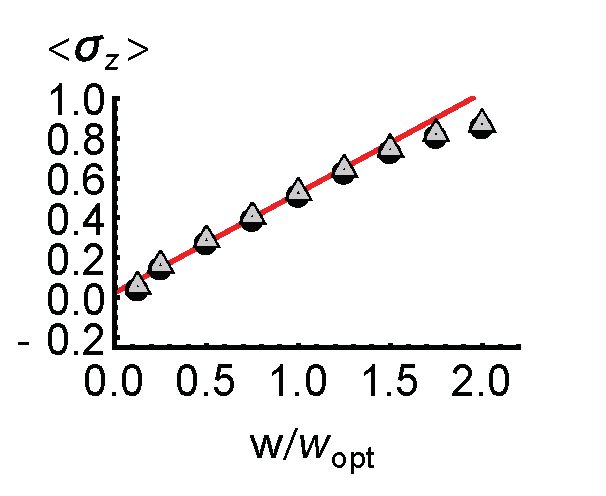
\includegraphics[scale =0.38] {N40SuperradianceSZ.eps}
	\hspace{-5.0mm} 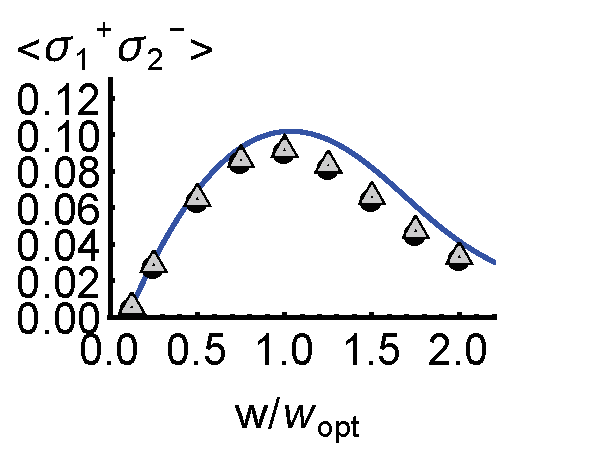
\includegraphics[scale =0.38] {N40SuperradianceSPSM.eps}
	\hspace{-5.0mm} 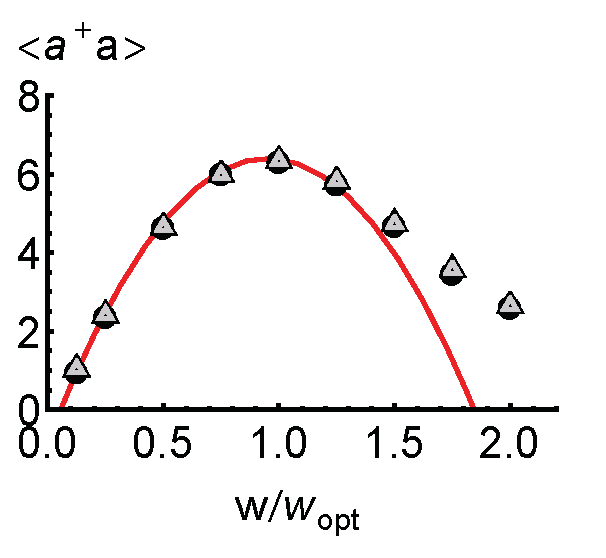
\includegraphics[scale =0.38] {N40Superradianceada.eps}
	\hspace{-5.0mm} 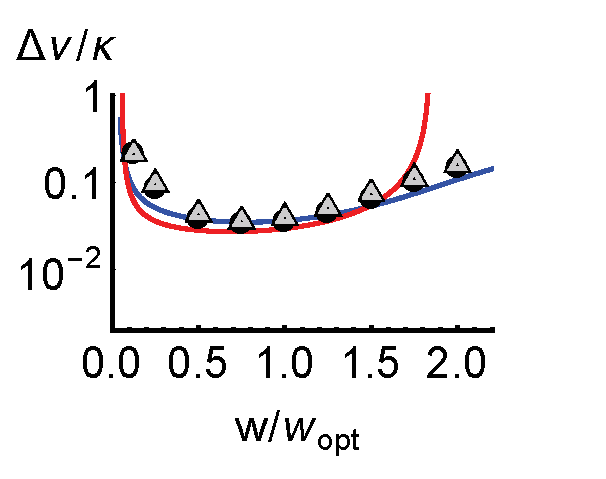
\includegraphics[scale =0.38] {N40SuperradianceLW.eps}
	\hspace{-5.0mm} 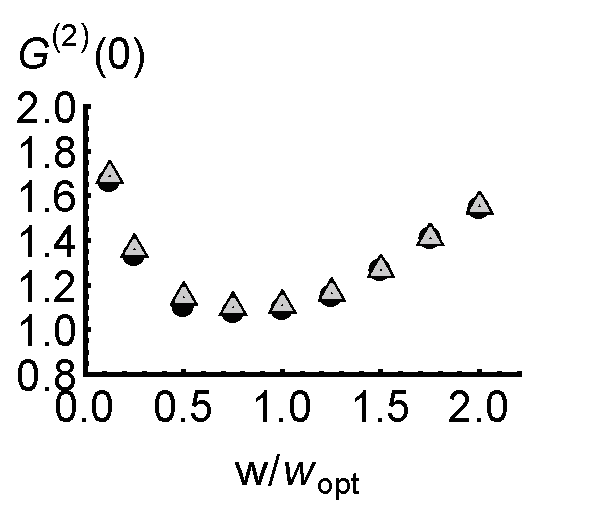
\includegraphics[scale =0.38] {N40SuperradianceG2.eps}\\ \vspace{0mm}
	\rotatebox{90}{ \hspace{7mm} \textbf{Crossover}}
	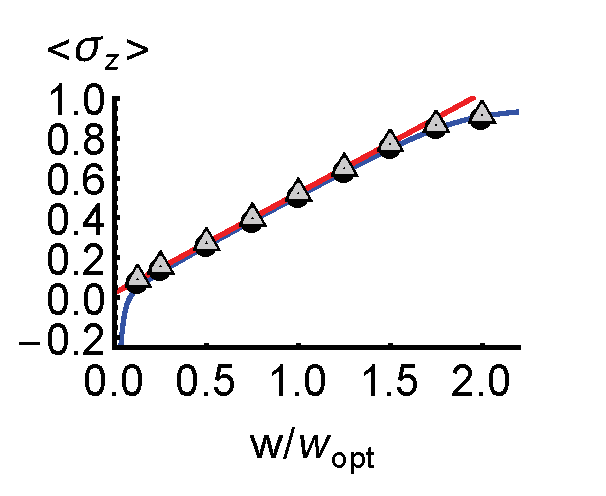
\includegraphics[scale =0.38] {N40CrossoverSZ.eps}
	\hspace{-5.0mm} 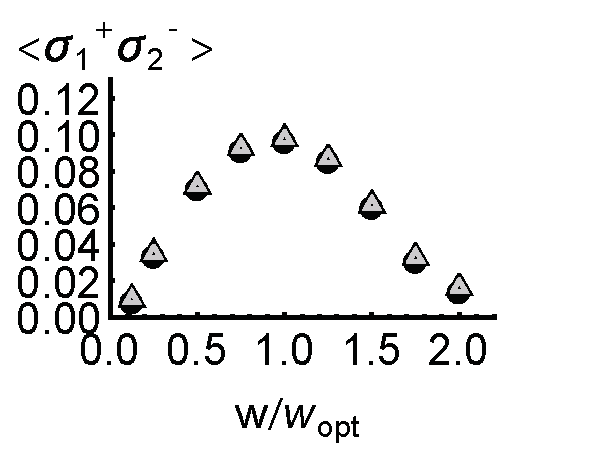
\includegraphics[scale =0.38] {N40CrossoverSPSM.eps}
	\hspace{-5.0mm} 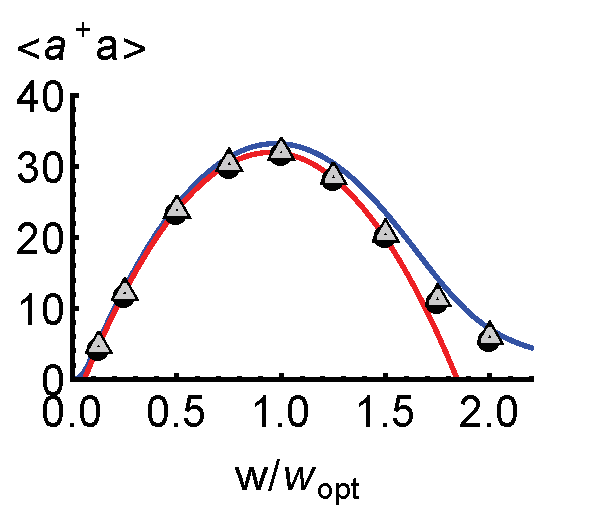
\includegraphics[scale =0.38] {N40Crossoverada.eps}
	\hspace{-5.0mm} 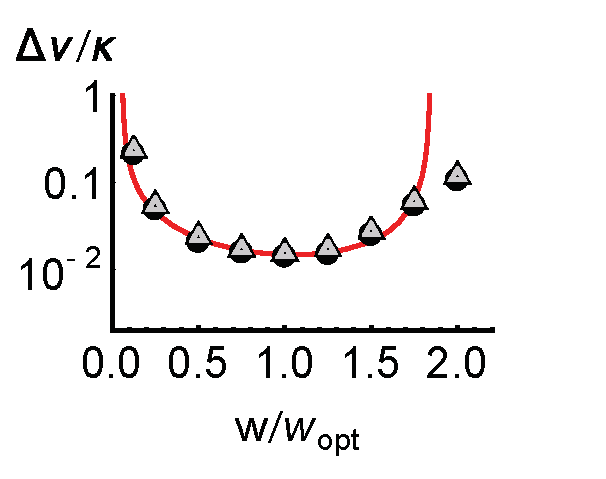
\includegraphics[scale =0.38] {N40CrossoverLW.eps}
	\hspace{-5.0mm} 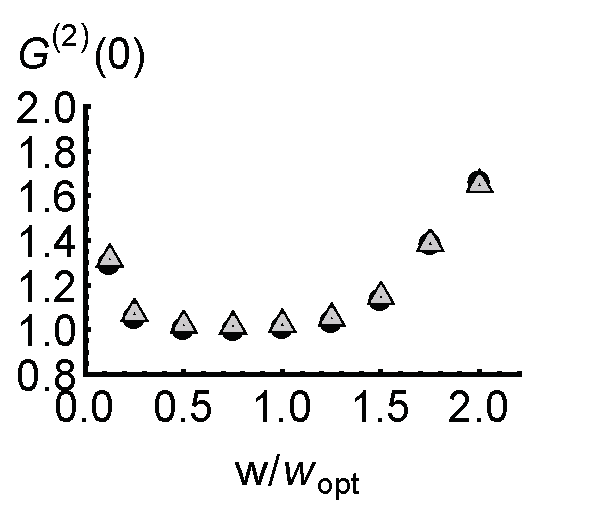
\includegraphics[scale =0.38] {N40CrossoverG2.eps}\\ \vspace{0mm}
	\rotatebox{90}{ \hspace{10mm} \textbf{Lasing}}
	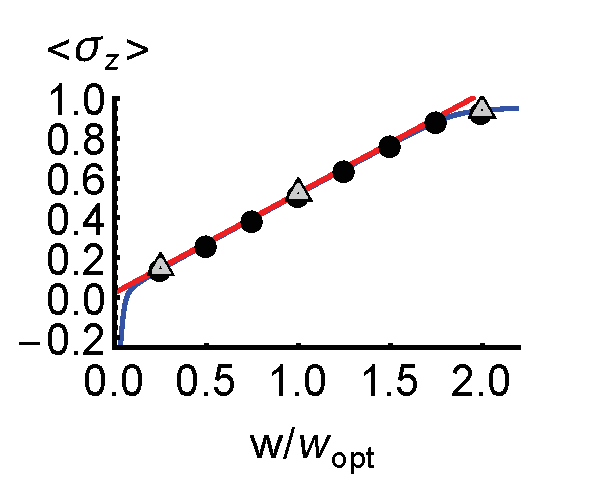
\includegraphics[scale =0.38] {N40LaserSZ.eps}
	\hspace{-5.0mm} 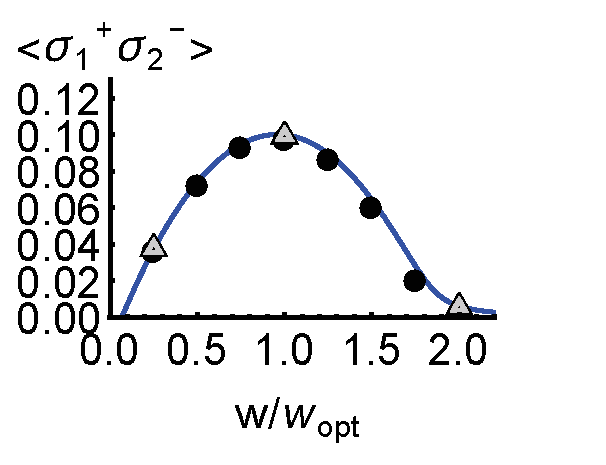
\includegraphics[scale =0.38] {N40LaserSPSM.eps}
	\hspace{-5.0mm} 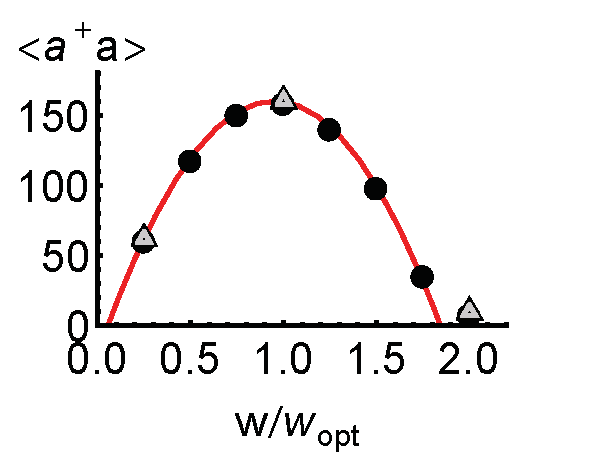
\includegraphics[scale =0.38] {N40Laserada.eps}
	\hspace{-5.0mm} 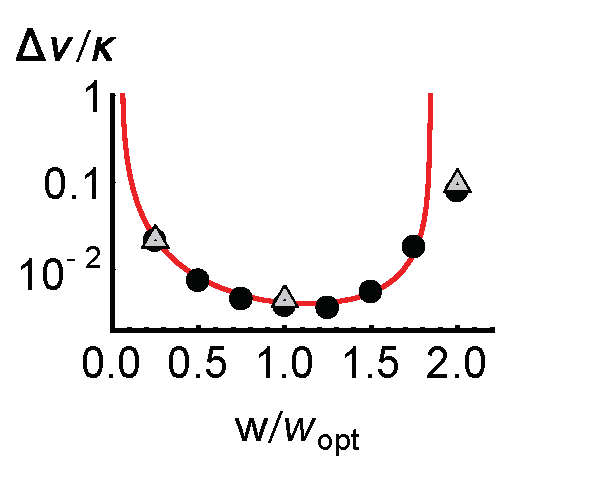
\includegraphics[scale =0.38] {N40LaserLW.eps}
	\hspace{-5.0mm} 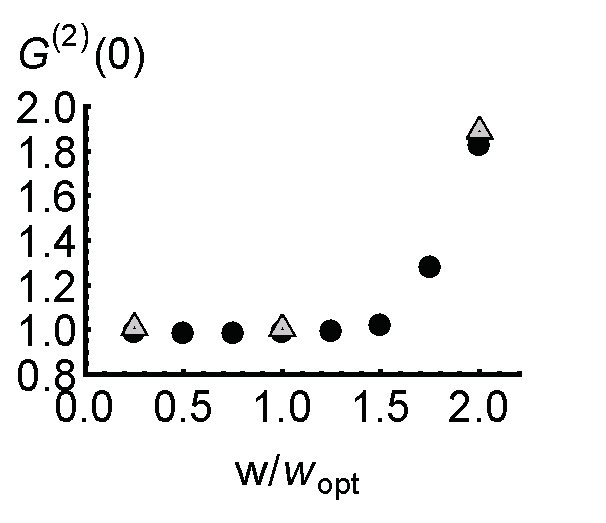
\includegraphics[scale =0.38] {N40LaserG2.eps}\\ \vspace{1mm}
	\hspace{5mm}(a)\hspace{30mm}(b) \hspace{30mm}(c) \hspace{30mm}(d) \hspace{30mm}(e)
\end{center}
		\vspace{-5mm}
\caption{(Color online) Comparison of the different solution methods in
the superradiance ($\xi=0.2$), crossover ($\xi=1$), and lasing ($\xi=5$)
regions for $N=40$ and $\frac{\Omega^2}{\kappa \gamma}=1$.  The analytic Langevin (phase diffusion and mean field) solutions are shown
in red (light gray), the 2nd order cumulant solutions are shown in blue
(dark gray), the exact SU(4) solution is shown by grey triangles, and the
{\it c}-number Langevin simulation results are shown by black circles. The
observables considered are (a) the inversion
$\left<\hat{\sigma}^{z}\right>$, (b) the correlation between the atoms'
dipoles
$\left<\hat{\sigma}_{1}^{+} \hat{\sigma}_{2}^{-}\right>$, (c) the
intracavity photon number  $\left<\hat{a}^{\dagger}\hat{a}\right>$, (d)
the linewidth $\Delta \nu$, and (e) the intensity correlation function
$G^{(2)}(0)$.}
\label{N40Comparison}
\end{figure*}


\subsection{Mean Field Equations}

By taking expectation values of the semi-classical equations
(\ref{cq1}-\ref{eqn:cnumberlangevin}) we obtain the so called mean field
equations

\begin{equation}
\frac{d}{dt} a_0= -\frac{1}{2} (\kappa +2i(\omega_c-\omega)) a_0
-\frac{i N \Omega}{2} S_0^{-},
\label{La0}
\end{equation}
\begin{equation}
\frac{d}{dt} S_0^{-} =
-\frac{1}{2} \left(\Gamma +2 i (\omega_a-\omega) \right)  S_0^{-}
+\frac{i \Omega}{2} \hat{a} S_0^{z},
\end{equation}
\begin{equation}
\frac{d}{dt} S_0^{z} = -(w+\gamma)\left( S_0^{z} - d_0\right)
+i\Omega \left( a_0^{\dagger} S_0^{-} - a_0 S_0^{+} \right)\;.
\label{Lsz0}
\end{equation}
The noise terms drop out because they have zero mean.
The mean field equations capture many of the most important features of the
physical system because the noise terms scale as $\sqrt{N}$ while the
expectation values scale as $N$.  In the limit of large numbers of atoms
the noise terms are therefore less important.  In equations
(\ref{La0}-\ref{Lsz0}) we have gone over to a reference frame rotating
at frequency $\omega$.

The mean field equations can be solved in closed form in steady state.
The steady state equations are obtained by setting the time derivatives
in Eqns.~(\ref{La0})~--~(\ref{Lsz0}) to zero.  We find
\begin{equation}
S_0^{z}=
\frac{(\kappa+2i(\omega_c-\omega))(\Gamma+2i(\omega_a-\omega))}{N\Omega^2}
\label{Sz01}
\end{equation}
for the steady state inversion.  Because $S_0^{z}$ must be real,
we find that oscillation frequency of the atom-cavity coupled system is
\begin{equation}
\omega = \frac{\kappa \omega_a + \Gamma \omega_c}{\kappa+\Gamma}\;.
\label{atomcavityfrequencycenter1}
\end{equation}
When $\delta = \omega_a-\omega_c \ll \Gamma,\kappa$ the inversion can be
simplified to
\begin{equation}
S_0^{z}\approx frac{1}{\mathcal{C}}\;,
\end{equation}
where $\mathcal{C}\equiv \frac{N \Omega^2}{\kappa \Gamma}$ is the
many-atom cooperativity parameter.  In the same limit of small detuning
we find for the steady state photon number
\begin{equation}
|a_0|^2=\frac{N(w+\gamma)}{2 \kappa} (d_0 - \frac{1}{\mathcal{C}})\;.
\label{a0sqSS}
\end{equation}
The photon number has a maximum at
\begin{equation}
w=w_{\mathrm{opt}} = \frac{N \Omega^2}{2\kappa} - \gamma - \frac{1}{T_2}.
\label{wopt}
\end{equation}
In the limit where the collective decay rate $\mathcal{C}\gamma$ is much
larger than the single atom decay rates $\gamma$ and $\frac{1}{T_2}$ we
find a simple expression for the maximum photon number,
\begin{equation}
(|a_0|^2)_{\mathrm{opt}}= \frac{N^2 \Omega^2}{8\kappa^2}\;.
\label{adaopt}
\end{equation}

The zeros of the intra cavity photon number Eq.~(\ref{a0sqSS}) determine
the thresholds of the system.  At the first threshold
\begin{equation}
w_1 = \gamma,
\label{FirstThreshold}
\end{equation} 
energy is supplied to the system at a high enough rate to sustain a
macroscopic field amplitude in the cavity.  The emergence of a coherent
macroscopic field amplitude is accompanied by the formation of a
collective atomic dipole.  A second threshold occurs at
\begin{equation}
w_2 =  \frac{N \Omega^2}{\kappa}\;.
\end{equation} 
At this point, $S_0^{z}$ is close to unity, and the noise due to the
strong repumping prevents the formation of a macroscopic coherent state
in the cavity and of a macroscopic dipole in the atomic ensemble.


\section{Characterization of the Crossover}
\label{sec:CrossoverCharacterization}

A characterization of the parameter space of a cavity QED system can
now be given. Since the repumping rate $w$ is varied in a typical
experiment, the system is characterized by considering the value
$w=w_{opt}$, at which there is a maximum number of intra-cavity
photons. We define a crossover parameter $\xi$ to be the ratio of the
modified atomic linewidth (including repumping $w$ and dephasing
$1/T_2$) evaluated at the optimum repump rate $w=w_{opt}$, to the
cavity linewidth $\kappa$,
\begin{equation}
\xi\equiv\frac{ w_{opt}+\gamma+\frac{1}{T_2}}{4\kappa}.
\label{CrossoverParameter}
\end{equation}
Inserting Eq.~(\ref{wopt}) into  Eq.~(\ref{CrossoverParameter}) yields,
\begin{equation}
\xi\equiv \frac{N \Omega^2}{8\kappa^2}.
\label{CrossoverParameter2}
\end{equation}
Eq.~(\ref{adaopt}) can then be used to rewrite $\xi$ in terms of
$(|a_0|^2)_{opt}$. We do this since it provides an alternative
interpretation of $\xi$ as a parameter that characterizes the
crossover, since,
\begin{equation}
\xi = \frac{(|a_0|^2)_{opt}}{N},
\end{equation}
{\em i.e.}\ it is proportional to the ratio of the intra-cavity photon
number to atom number. Thus one may interpret $\xi$ as a quantity that
expresses the relative importance of stimulated emission to collective
atomic effects. If $\xi\ll1$, the system is in the bad cavity or superradiant
regime. If $\xi\gg1$ the system is in the good cavity or laser
regime. The region $\xi\sim1$ defines the intermediate or crossover regime.


\section{Results}
\label{sec:Results}

\begin{figure*}
\begin{center}
	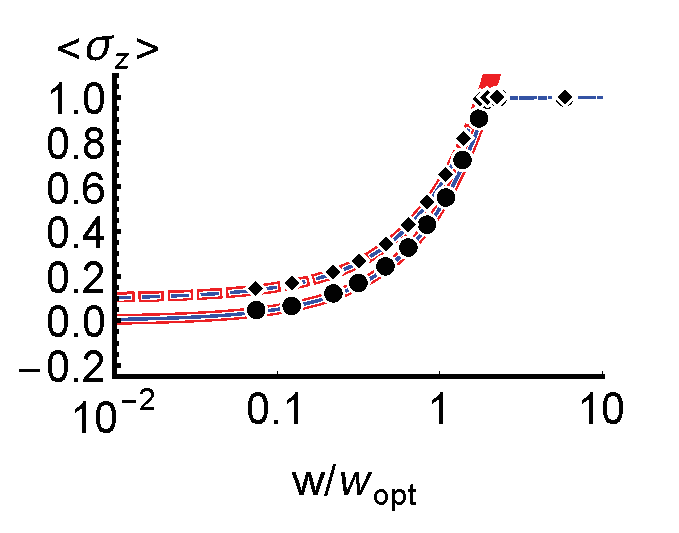
\includegraphics[scale =0.445] {N10000SZ.eps}
	\hspace{-5.0mm} 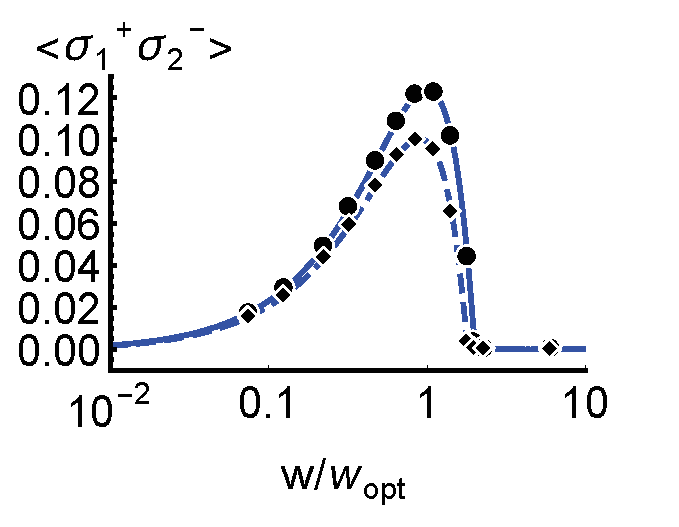
\includegraphics[scale =0.445] {N10000SPSM.eps}
	\hspace{-6.5mm} 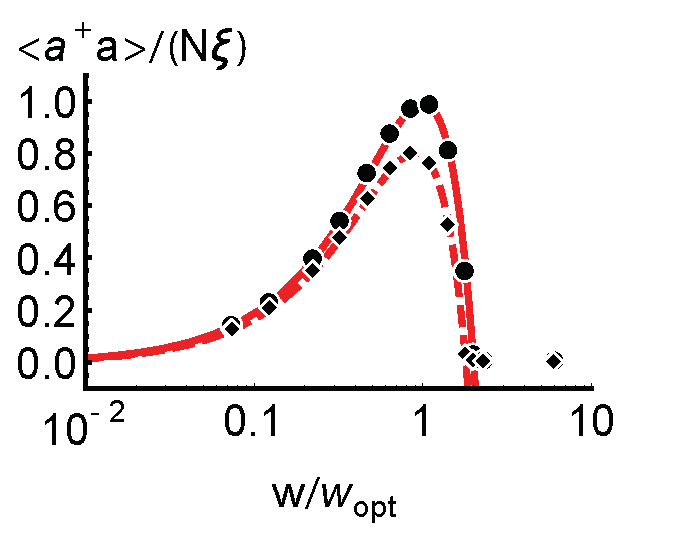
\includegraphics[scale =0.445] {N10000ada.eps}
	\hspace{-5.5mm} 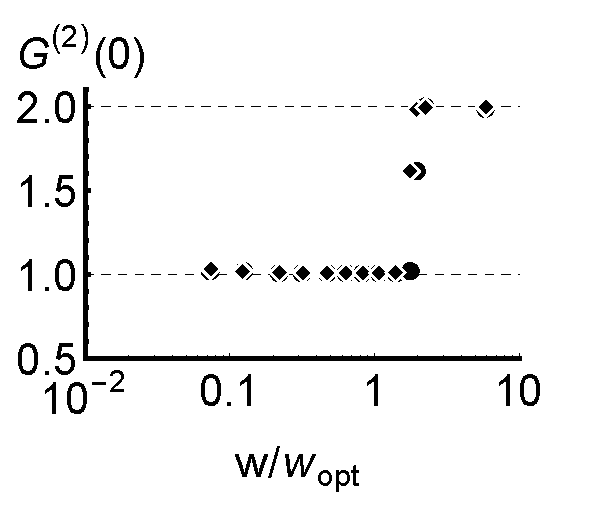
\includegraphics[scale =0.445] {N10000G2S.eps}\\
	\textbf{(a) Universal}\\
	\line(1,0){500}\\
	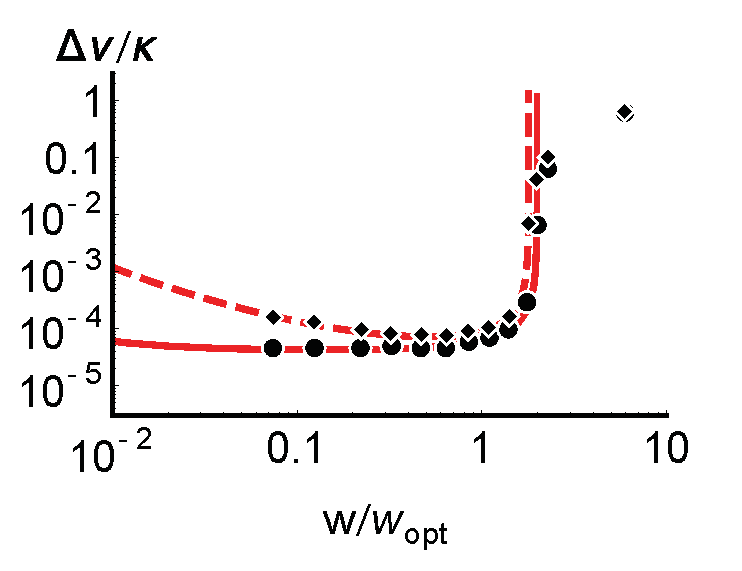
\includegraphics[scale =0.51] {N10000LWS.eps}
	\hspace{-5.5mm} 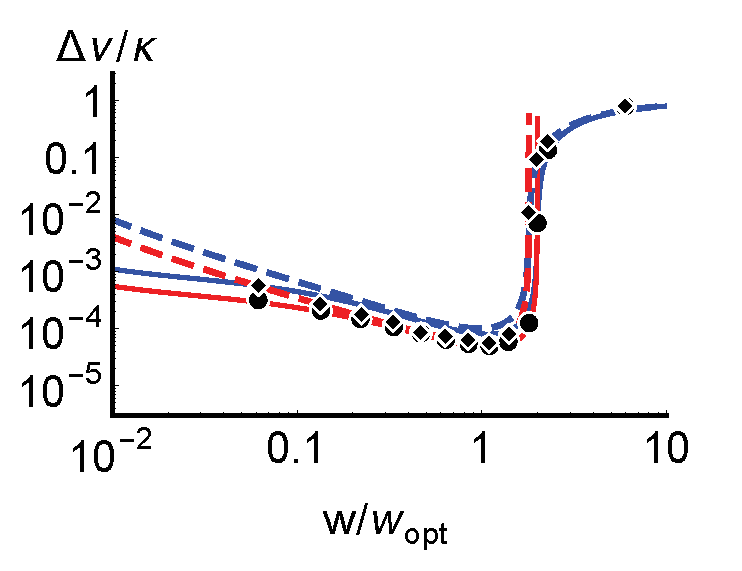
\includegraphics[scale =0.51] {N10000LWC.eps}
	\hspace{-5.5mm} 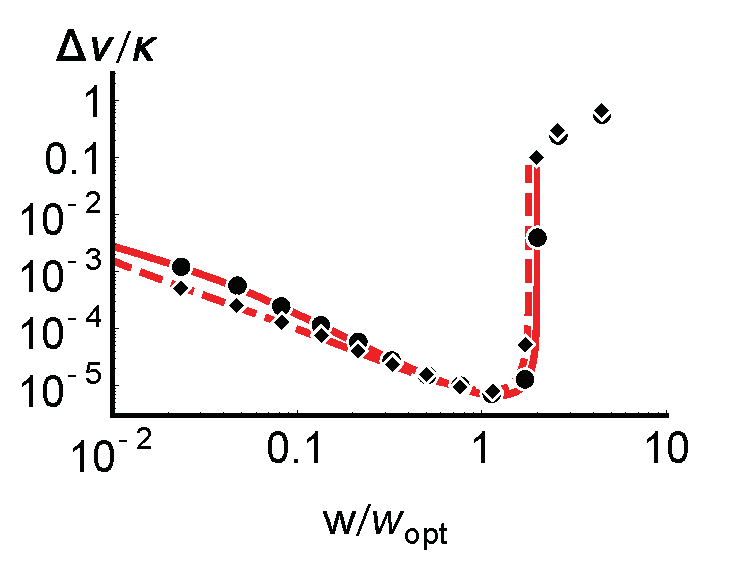
\includegraphics[scale =0.51] {N10000LWL.eps}\\
	\hspace{-10mm}\textbf{(b) Superradiance}\hspace{33mm}\textbf{(c) Crossover}
  \hspace{37mm}\textbf{(d) Lasing}
\end{center}
		\vspace{-5mm}
\caption{(Color online) Solutions using the various methods in the
superradiance ($\xi=0.1$), crossover ($\xi=1$), and lasing ($\xi=10$)
regions for N=10000 and $\frac{\Omega^2}{\kappa \gamma}=0.1$. For $1/T_2=0$, the analytic Langevin (phase diffusion and mean field) solutions are shown in solid red (solid light gray), the 2nd order
cumulant solutions are shown in solid blue (solid dark gray), and the
{\it c}-number Langevin simulation results are shown by black circles. For
$1/T_2=\frac{1}{5} w_{opt}$, the analytic Langevin solutions are shown in
dashed red (dashed light gray), the 2nd order cumulant solutions are shown
in dashed blue (dashed dark gray), and the {\it c}-number Langevin simulation
results are shown by black diamonds. (a) All observables considered
except linewidth  $\Delta \nu$ show universal behavior in the
superradiance, crossover, and lasing regions, after appropriate scaling.
The red (light gray) curves have been artificially widened in order to
be seen underneath the blue curves. (b)  $\Delta \nu / \kappa$ in the
superradiance region (c) $\Delta \nu / \kappa$ in the crossover region,
(d) $\Delta \nu / \kappa$ in the lasing region.}
 \label{N10000Comparison}
\end{figure*}


\subsection{Simulations with $N=40$}

In order to determine the validity of the approximate solution methods, we begin by comparing them to the exact solutions. This comparison is done for $N=40$, since this is a small enough number of atoms that the exact method can be used, and large enough to expect the approximate solution methods to be reasonably accurate. 

Specifically, the mean field Langevin method, the phase diffusion method, the {\it c}-number Langevin method, and the 2nd order cumulant method are compared to the exact SU(4) result for three different values of the crossover parameter:
$\xi=0.2$, $\xi=1$, and $\xi=5$. These values of $\xi$ put the system in the
superradiance, crossover, and lasing parameter regions, respectively.
This comparison can be seen in Fig.~\ref{N40Comparison}. We note that the SU(4) method becomes more computationally intensive as $\xi$ is increased, since there are more photons as $\xi$ is increased, and hence
more basis states need to be tracked. Therefore, for $\xi=5$, the method
that combines the SU(4) with quantum jump method was used (see Appendix~\ref{Su4Appendix}). This
simulation is computationally intensive, so that only a few values of $w$
are included.

Fig.~\ref{N40Comparison} shows that there is an excellent agreement
between {\it c}-number Langevin and the exact SU(4) theory for $N=40$, in all
parameter regions, for all of the considered observables. Therefore, the
{\it c}-number Langevin theory can be relied upon for larger atom numbers,
where it is not possible to apply the SU(4) theory.

The 2nd order cumulant solution works well qualitatively in all
parameter regions, but as seen in Fig.~\ref{N40Comparison} (b) and (c)
in the superradiance row, and in column (d), there is a quantitative
disagreement between this theory and the SU(4) and {\it c}-number Langevin
theories. This quantitative disagreement is due to the fact that a theory which factorizes all moments
into products of no higher than second order, and a theory that
uses Gaussian noise are not equivalent. This difference can be seen by considering the
third order moment $\left< \hat{a}^{\dagger}\hat{a}\hat{\sigma}_i^z
\right>$. According to the cumulant theory, $\left<
\hat{a}^{\dagger}\hat{a}\hat{\sigma}_i^z \right>=\left<
\hat{a}^{\dagger}\hat{a}\right> \left<\hat{\sigma}_i^z \right>$, a fact
which was essential to use in deriving the closed the set of equations
used to find the spectrum \cite{PhysRevLett.102.163601}. In the Langevin
theory, however, $\left< \hat{a}^{\dagger}\hat{a}\hat{\sigma}_i^z
\right> \neq \left< \hat{a}^{\dagger}\hat{a}\right>
\left<\hat{\sigma}_i^z \right>$, a fact we have checked with our
Langevin simulations. Even though the difference between $\left<
\hat{a}^{\dagger}\hat{a}\hat{\sigma}_i^z \right>$ and $\left<
\hat{a}^{\dagger}\hat{a}\right> \left<\hat{\sigma}_i^z \right>$
decreases as $\frac{1}{N}$, it is precisely the $\frac{1}{N}$ terms that
gives rise to the linewidth according to the cumulant theory.  Therefore
the $25\%$ disagreement between the Langevin and cumulant theories for
large N is not surprising.

Seen in Fig.~\ref{N40Comparison} (a) and (c), the mean field Langevin method
works well in the region around $w/w_{opt}=1$, but disagrees outside that region. In Fig.~\ref{N40Comparison} (d),
it can be seen that the phase diffusion model for the linewidth also agrees in the region around $w/w_{opt}=1$, but disagrees outside that region, where the phase diffusion approximation breaks down. 

Although they do not qualitatively agree with the SU(4) method, the analytic solutions yielded by the mean field, phase diffusion and second order cumulant theories capture the correct qualitative behavior of the system.


\subsection{Simulations with $N=10000$}

Now that an agreement between the {\it c}-number Langevin and exact SU(4)
theories has been established, we study more experimentally realistic
systems with $N=10000$ by applying {\it c}-number Langevin theory. We also
include the mean field Langevin theory, the phase diffusion model for the linewidth, and the 2nd order cumulant theory for
reference. The results of these simulations can be seen in
Fig.~\ref{N10000Comparison}. Both the situation in which $1/T_2=0$ and
in which $1/T_2=w_{opt}/5$ are considered.

As seen in Fig.~\ref{N10000Comparison} (a), when $1/T_2=0$, the
inversion $\left<\hat{\sigma}^{z}\right>$, the correlation between atoms
$\left<\hat{\sigma}_{1}^{+} \hat{\sigma}_{2}^{-}\right>$, the
intracavity photon number  $\left<\hat{a}^{\dagger}\hat{a}\right>$,  and
the intensity correlation function $G^{(2)}(0)$ all show universal
behavior in the superradiance, crossover, and lasing regimes after
appropriate scaling. When $1/T_2$ is large, $1/T_2=w_{opt}/5$, these
observables still show universal behavior after appropriate scaling, and
the values do not change significantly from the $1/T_2=0$ case.

It is worth noting that even though  $\left<\hat{\sigma}_{1}^{+}
\hat{\sigma}_{2}^{-}\right>$ has universal behavior throughout the
crossover, typical lasers are operated just above threshold at $w \ll
w_{opt}$, where the resulting value of
$\left<\hat{\sigma}_{1}^{+}\hat{\sigma}_{2}^{-}\right>_{opt}$ is much
smaller, so that atom-atom correlations are not important in lasers operating in the conventional regime.

The linewidth $\Delta \nu$, however, does not show universal behavior in the superradiance, crossover, and lasing regimes. As seen in Fig.~\ref{N10000Comparison} (b), in the superradiance region, when $1/T_2=0$, $\Delta \nu / \kappa$ is flat in the region of $w/w_{opt}<1$. In contrast, the linewidth in the lasing regime, shown in Fig.\ref{N10000Comparison} (d), linearly decreases as $w/w_{opt}$ increases towards unity. This is the typical Schawlow-Townes behavior, which can be seen by considering $\kappa/\left<\hat{a}^{\dagger}\hat{a}\right>$ using Eq.~\ref{a0sqSS}. In the crossover region, shown in Fig.~\ref{N10000Comparison} (c), we see that for $w/w_{opt}$ small, $\Delta \nu/\kappa$ is flat, and as $w/w_{opt}$ approaches unity, $\Delta \nu/\kappa$ starts to linearly decrease as in the lasing regime. Therefore, a system in the crossover region displays characteristics of both superradiance and lasing. 

When $1/T_2$ is increased to $1/T_2=w_{opt}/5$,
Fig.~\ref{N10000Comparison} (b) shows that $\Delta \nu/\kappa$ is
increased for $w/w_{opt}$ small, but it is not significantly affected by
$1/T_2$ as $w/w_{opt}$ approaches unity. In any case, this is the region
in which a superradiant system should be operated, since this is the
region of maximum intracavity intensity.

In the crossover region, seen in Fig.~\ref{N10000Comparison} (c), when
$1/T_2=w_{opt}/5$, $\Delta \nu/\kappa$ is increased for $w/w_{opt}$
small, where the system is displaying superradiant behavior, but is
completely insensitive to $w/w_{opt}$ approaching unity, where the
system starts to display lasing behavior.

As seen in Fig.~\ref{N10000Comparison} (d), in the lasing region, when
$1/T_2=w_{opt}/5$, $\Delta \nu/\kappa$ is not increased, but actually
decreased in the region slightly below $w/w_{opt}=1$, when compared to
the $1/T_2=0$ case. This reduction has also been observed for smaller
atom numbers using the exact SU(4) code. It can be shown that the value
of $1/T_2$ that maximally reduces the linewidth is
$1/T_2=\frac{w_{opt}}{1+\sqrt{2}}$.

A typical laser is operated just above threshold, where $w/w_{opt} \ll
1$. As seen in Fig.~\ref{LWadaComparison} (a), for the same pump
strength $w$, and a fixed $N$, a system in the crossover region could be
operated with $w/w_{opt} = 1$, allowing the crossover system to have a
linewidth orders of magnitude smaller than the linewidth of the lasing
system. Fig.~\ref{LWadaComparison} (b) shows that the intracavity
intensity, $\left<\hat{a}^{\dagger}\hat{a}\right>$, will be roughly the
same for the crossover system operated at $w/w_{opt} = 1$ as for a laser
system operated at  $w/w_{opt} \ll 1$.

\begin{figure}
\begin{center}
	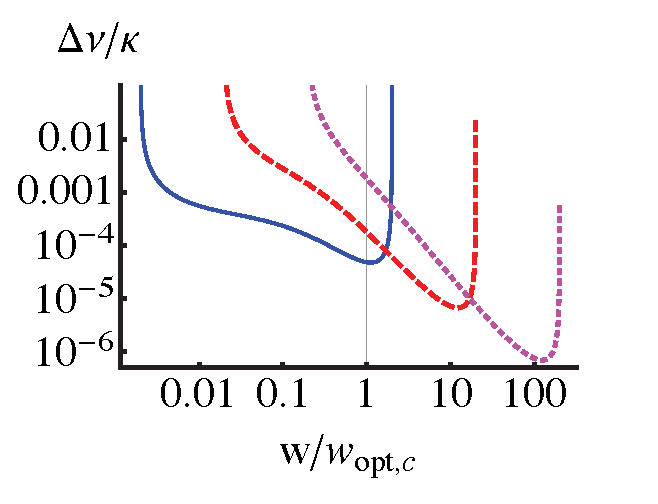
\includegraphics[scale =0.415] {LinewidthComparisonLangevin.eps}
	\hspace{-4mm} 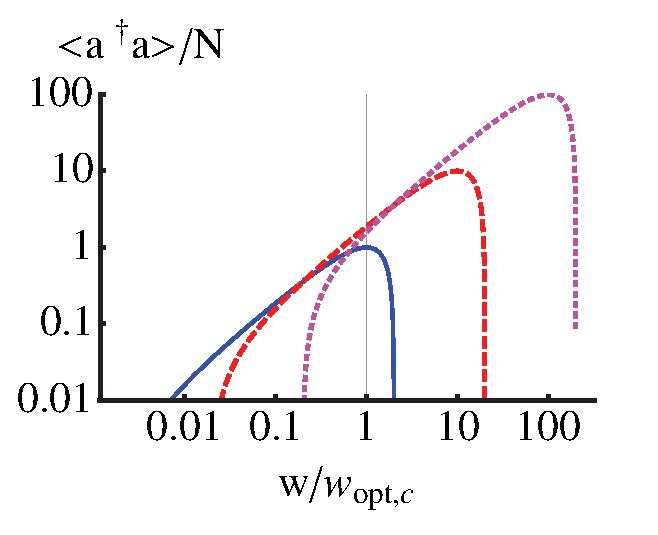
\includegraphics[scale =0.415] {adaComparisonLangevin.eps}\\
	\hspace{6mm}\textbf{(a)}\hspace{37mm}\textbf{(b)} \hspace{35mm}
\end{center}
		\vspace{-5mm}
\caption{(Color online) Comparison of (a) linewidth and (b) Intracavity
intensity for a system operated in the crossover ($\xi=1$) shown in blue
solid, lasing ($\xi=10$) shown in red dashed, and far lasing ($\xi=100$)
shown in magenta dotted, regions using the analytic (phase diffusion and mean field) Langevin model. $w_{opt,c}$ is the optimum $w$ value
in the crossover region. For all systems, $N=10000$ and $\frac{\Omega^2}{\kappa \gamma}=0.1$.}
\label{LWadaComparison}
\end{figure}

\subsection{Effect of Cavity and Atomic Level Instabilities on the
Spectrum}

The effect of instabilities in the cavity frequency and atomic frequency
on the linewidth is now investigated. Cavity frequency instability can
be caused by fluctuations in cavity length due to the thermal
fluctuations of the cavity mirrors, which are unavoidable in an
experiment. The energy levels in an atom can also be shifted by stray
electromagnetic fields. The frequency of the combined atom-cavity system
$\omega$ lies somewhere between the bare atom and cavity frequencies,
and is given by Eq.~(\ref{atomcavityfrequencycenter1}).

If $\omega$ is varied, the resultant time averaged linewidth will be an
average over these values, and will hence be much broader than the
quantum limited linewidth. Therefore, the derivative of  $\omega$ with
respect to $\omega_c$, and with respect to $\omega_a$, gives us an idea
as to how much of an effect an instability in these frequencies will
have on broadening the linewidth. These derivatives are plotted in
Fig.~\ref{CavityInstability}.

Fig.~\ref{CavityInstability} (a) tells us that on the lasing side of the
crossover, $\omega$ is shifted proportionally to the shift in
$\omega_c$, while on the superradiant side, $\omega$ is insensitive to
shifts in $\omega_c$.  Conversely, in Fig.~\ref{CavityInstability} (b)
it can be seen $\omega$ is shifted proportionally to the shift in
$\omega_a$ on the superradiance side of the crossover, while on the
lasing side, $\omega$ is insensitive to shifts in $\omega_a$. In the
intermediate regime ($\xi=1$), $\omega$ is not as sensitive to a shift
in the $\omega_c$ as it is in the laser regime, and it is not as
sensitive to a shift in the $\omega_a$, as it is on the superradiance
side.

\section{Conclusion}

A model that is capable of describing a system operating in any
parameter region of the crossover between steady state superradiance and
lasing was introduced. Since this model can only be solved exactly for small systems, several solution methods that treat the quantum fluctuations with varying degree of approximation were introduced, based on the property that in these systems, fluctuations scale inversely with the number of particles.  First, mean field equations, which neglect all quantum fluctuations, were used to derive analytic expressions for many of the system observables. These analytic expressions were used to motivate the definition of the crossover parameter. Since the mean field equations cannot describe the spectral properties of the system, the method {\it c}-number Langevin equations with Gaussian fluctuations was introduced. For small systems, where the exact SU(4) method can be applied, the {\it c}-number Langevin method showed excellent agreement with the exact SU(4) method. Therefore, the {\it c}-number Langevin method was used to treat larger systems, and a comparison of the properties of systems operating in the different parameter regions of the crossover was made. 

\begin{figure}
\begin{center}
	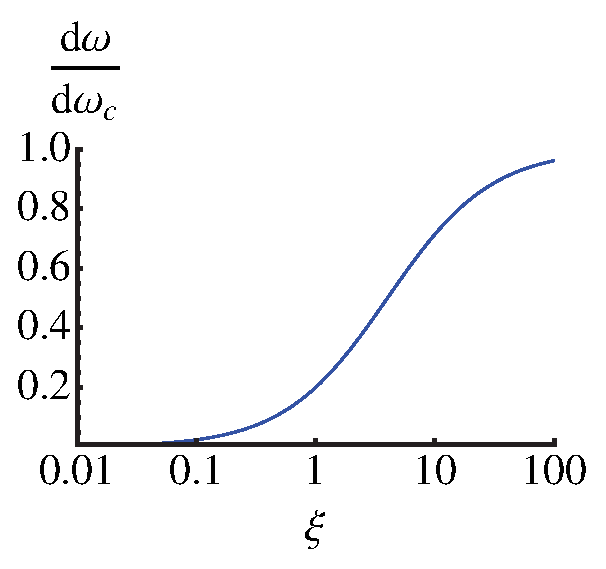
\includegraphics[scale=0.42] {CavityInstability.eps} \hspace{2mm}
	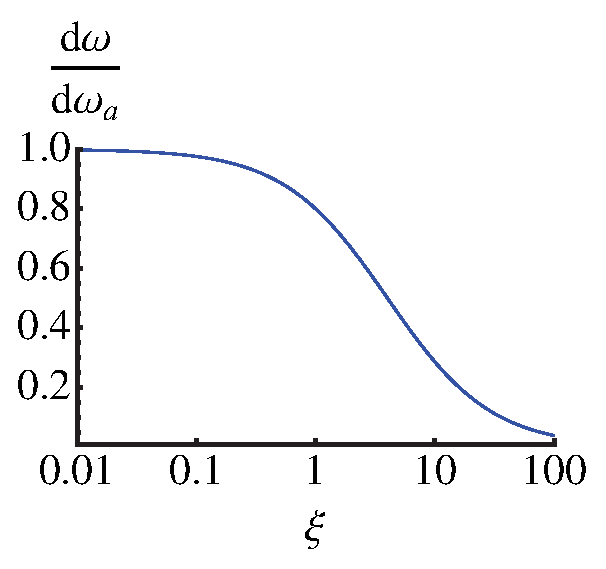
\includegraphics[scale=0.42] {AtomInstability.eps}\\
\hspace{2mm} \textbf{(a)}\hspace{40mm}\textbf{(b)} \hspace{35mm}
\end{center}
\caption{(Color online) Instability in the atom-cavity system frequency
$\omega$ with respect to (a) the cavity frequency $\omega_c$ and (b)
atomic frequency $\omega_a$ as a function of crossover parameter $\xi$. These results were calculated using Eq.~(\ref{atomcavityfrequencycenter1}).}
\label{CavityInstability}
\end{figure}

Although a system in the lasing parameter region is capable of
possessing the smallest linewidth, typically lasers operate with a
re-pumping rate that puts them just above threshold, which does not
allow the smallest linewidth for the system to be realized. For the same
re-pumping rate, a system operating in the crossover region will be
farther above threshold, potentially allowing for a linewidth orders of
magnitude smaller than in the laser region. Also, a crossover system
will have a larger intracavity intensity than a superradiant system,
making the former more experimentally accessible.

It was also demonstrated that a system in all regions of the crossover
is insensitive to atomic dephasing as long as the re-pumping rate is
smaller than the dephasing rate. Also, as the crossover is traversed
into the lasing region, atomic dephasing can actually cause a reduction
in the linewidth.

Finally, it was shown that the linewidth on the superradiance side is
insensitive to fluctuations in cavity length, and that these
fluctuations become more important as the crossover is traversed toward
the laser side. Conversely, it was shown that the linewidth on the
lasing side is insensitive to fluctuations in the atomic energy levels,
and that these fluctuations become more important on the superradiance
side. A system in the crossover region will be less sensitive to cavity
frequency fluctuations than a lasing system, and it will be less
sensitive to atomic frequency instabilities than a superradiant system.
Both of these fluctuations cause a broadening of the linewidth. These
conclusions are significant since fluctuations in the cavity frequency
are a principal limitation preventing further reduction of the linewidth
in today's most ultrastable lasers.

This work has been supported by JILA-NSF-PFC-1125844, DARPA, QuASAR, and
NIST.

\appendix

\section{SU(4) Numerical Simulation of the Master Equation}
\label{Su4Appendix}

Recently, we have developed a group-theoretic method for efficiently
simulating the quantum master equation~\cite{PhysRevA.87.062101}. In brief, the
master equation, Eq.~(\ref{ME1Crossover}), can be expressed in terms of
generators of the SU(4) group, with the Hamiltonian part being,
\begin{eqnarray}
  &&\frac{1}{i\hbar}[H,\rho]=
  -2i \omega_a \Sigma_3\rho -i\omega_c [ \hat{a}^{\dagger}\hat{a}, \rho]
  \nonumber
  \\
  &&-i\Omega \left[a(\mathcal{M}_++\mathcal{N}_+)\rho+a^\dagger
    (\mathcal{M}_-+\mathcal{N}_-)\rho\right]\nonumber\\
  &&\quad{}+i\Omega\left[(\mathcal{U}_++\mathcal{V}_+)\rho a^\dagger
    +(\mathcal{U}_-+\mathcal{V}_-)\rho a\right]\,,
\end{eqnarray}
and dissipation parts being,
\begin{eqnarray}\label{liv}
 && \sum_{j=1}^N(
   2\sigma_j^-\rho\sigma_j^+-\sigma_j^+ \sigma_j^-\rho-
   \rho \sigma_j^+\sigma_j^-
  )/2=-\frac{N}{2}-
  \mathcal{Q}_3+\mathcal{Q}_{-}\,,\nonumber\\
 && \sum_{j=1}^N(
   2\sigma_j^+\rho\sigma_j^--\sigma_j^- \sigma_j^+\rho-
   \rho \sigma_j^-\sigma_j^+
  )/2=-\frac{N}{2}+
  \mathcal{Q}_3+\mathcal{Q}_{+}\,,\nonumber\\
 && \sum_{j=1}^N(\sigma_j^{(3)}\rho\sigma_j^{(3)}-\rho)=4\mathcal{M}_3-2
  \mathcal{Q}_3-2\Sigma_3-N\,,
  \label{ham}
\end{eqnarray}
where $\mathcal{Q}_{\pm}$, $\mathcal{M}_{\pm}$, $\mathcal{N}_{\pm}$,
$\mathcal{U}_{\pm}$, $\mathcal{V}_{\pm}$, $\mathcal{Q}_3$, $\mathcal{M}_3$,
and $\Sigma_3$ are superoperators~\cite{PhysRevA.87.062101}.  As a result, we can
expand the density matrix in terms of the fully symmetrical multiplet
$P_{q,q_3,\sigma_3}$~\cite{PhysRevA.87.062101} of the SU(4) group,
\begin{equation}\label{ex}
  \rho=\sum_{q,q_3,\sigma_3,m,n} C_{q,q_3,\sigma_3}^{m,n}
  P_{q,q_3,\sigma_3}\bigl|m\bigr>\bigl<n\bigr|\,,
\end{equation}
where $C_{q,q_3,\sigma_3}^{m,n}$ are complex coefficients, and
$|n\rangle$ is the photon Fock state. Note that the total number of
states in the fully symmetrical multiplet is $1/6 (N+1)(N+2)(N+3)$,
which reduces the exponential scaling of the problem to cubic in $N$.
This has enabled us to numerically investigate large
systems~\cite{PhysRevA.87.062101}.

However, the number of basis in Eq.~(\ref{ex}) also grows as square of
the photon number.  This would impose great difficulties in numerical
simulations of the laser region due to the large number of photons.
Below, we present a method that unravels the master equation in the
Liouville space, which enables us to remove the photon basis in the
simulation. The essential idea behind the method is that we are able to
deduce the photon state by keeping track of the total number of quanta
$N_q$ in the system.

The quantum Monte Carlo method decomposes the density operator evolution
into a set of quantum trajectories where, between applications of random
jumps into random channels, the system evolves under an effective
Hamiltonian~\cite{Dalibard92,Dum92,Knight98}. These random jumps are chosen with the proper weights, so that when many trajectories are averaged over, the correct density operator evolution is given. While this has
conventionally been done with wavefunctions to reduce the numerical
complexity, here we apply the quantum trajectory algorithm in the
density matrix space in order to get rid of the photon basis in the
expansion of the density operator. To construct a single trajectory, we
first need to identify the jump operators. In our problem, there are
four decay channels: repumping, spontaneous emission, dephasing and
cavity decay. The corresponding jump operators $\mathcal{J}_i$ are
\begin{eqnarray}
\mathcal{J}_1\rho&=&
w\sum_{j=1}^N(\sigma_j^+\rho\sigma_j^-)=w\mathcal{Q}_{+}\rho\,,
\nonumber\\
\mathcal{J}_2\rho&=&
\gamma\sum_{j=1}^N(\sigma_j^-\rho\sigma_j^+)=
\gamma \mathcal{Q}_{-}\rho\,,\nonumber\\
\mathcal{J}_3\rho&=&
\frac{1}{2T_2}\sum_{j=1}^N(\sigma_j^{(3)}\rho\sigma_j^{(3)})
\nonumber\\
&=&\frac{1}{2T_2}(4\mathcal{M}_3-2  \mathcal{Q}_3-2\Sigma_3)\rho\,,
\nonumber\\
\mathcal{J}_4\rho&=&\kappa a\rho a^{\dagger}\,.
\label{jumpo}
\end{eqnarray}
When a repumping quantum jump happens, $N_q$ is decreased by one. When a
spontaneous emission or a cavity-decay quantum jump happens, $N_q$ is
increased by one. The dephasing quantum jump also does not change the
total number of quanta. Therefore, during the evolution of a single
trajectory, one could calculate $N_q$ at every time step by tracking the
the numbers of jumps of the different types. With the knowledge of
$N_q$, the photon state can be easily deduced. It is shown in
Ref.~\cite{PhysRevA.87.062101} that
\begin{equation}
\begin{split}
  \hat{J}_3P_{q,q_3,\sigma_3}^{(\mathrm{s})}&=
  (q_3+\sigma_3)P_{q,q_3,\sigma_3}^{(\mathrm{s})},\\
  P_{q,q_3,\sigma_3}^{(\mathrm{s})}\hat{J}_3&=
  (q_3-\sigma_3)P_{q,q_3,\sigma_3}^{(\mathrm{s})},
\end{split}
\end{equation}
where $\hat{J}_3=\sum_{j=1}^N\sigma_j^{(3)}/2$ is the collective spin
operator. Therefore, the atomic state for a particular fully symmetrical
atomic basis in terms of the number of excited atoms is
$|q_3+\sigma_3+N/2\rangle\langle q_3-\sigma_3+N/2|$. And thus the
corresponding photon state is
\begin{equation}
\bigl|m\bigr>\bigl<n\bigr|=
\bigl|N_q-(q_3+\sigma_3+N/2)\bigr>
\bigl<N_q-(q_3-\sigma_3+N/2)\bigr|.
\end{equation}
Therefore, if the system starts in a photon number state, by counting the quantum jumps, we have complete knowledge of
photon states for every single trajectory. This enables us to remove the
photon basis, which greatly improves the efficiency of the method. 

The simulation of jump times and jump channels is completely analogous
to the wave-function Monte Carlo method. The effective evolution of the
system is governed by the master equation excluding the above jump
operators. As a result, under the effective evolution, the trace of the
density operator is no longer conserved, but decreases as a function of
time.  This is analogous to the decay of the norm of the wavefunction in
the wave function Monte Carlo method. A jump occurs when the trace of
the density operator is less than a random number uniformly distributed
in the interval $[0,1]$. When a decay occurs we stochastically determine
the channel $i$ into which the system decays according to the
probability distribution,
\begin{equation}
\mathcal{P}_i^{\mathrm{jump}}=\frac{\mathrm{Tr}[\mathcal{J}_i\rho]}{\sum_{k=1}^4
\mathrm{Tr}[\mathcal{J}_k\rho]}.
\end{equation}

Finally, in order to get the density operator at each time step, an
ensemble average of many quantum trajectories is required. Then, various
observables can be calculated according to Ref.~\cite{PhysRevA.87.062101}. It is
also worth noting that if one is only interested in the steady state
density operator, a time average in the steady state can be applied
instead of the ensemble average.

\section{Phase Diffusion Linewidth}
\label{HakenAppendix}

The linewidth due to the phase fluctuations of $\hat{a}$ is derived from the quantum Langevin equations, Eqns.~(\ref{La})~--~(\ref{Lsz}). Following closely to the derivation done in \cite{HakenLaser,
HakenLaserBook}, Eq.~(\ref{La}) is differentiated, and substituted into
it Eqns.~(\ref{La})~--~(\ref{Lsm}) and the integral of Eq.~(\ref{Lsz}), to
arrive at an equation for $\hat{a}$ alone,
\begin{equation}
\ddot{\hat{a}} =
-\frac{1}{2} (\kappa+\Gamma)  \dot{\hat{a}} -
\frac{\kappa \Gamma}{4}\hat{a}  +
\frac{N \Omega^2 }{4} \hat{a} \hat{S}^z +\hat{F},
\label{addeq}
\end{equation}
where
\begin{eqnarray}
\hat{S}^z &=&
\int_0^t dt^{\prime} e^{-(w+\gamma)(t-t^{\prime})}
\bigg( (w+\gamma) + \hat{F}^z
\nonumber
\\
&&\hspace{-3mm}-\frac{2}{N} \left( \frac{d}{dt} (\hat{a}^{\dagger} \hat{a}) +
\kappa \hat{a}^{\dagger} \hat{a} -\hat{a}^{\dagger} \hat{F}^a -
\hat{F}^{a^{\dagger}} \hat{a} \right) \bigg),
\end{eqnarray}
and,
\begin{equation}
\hat{F} = \frac{\Gamma}{2} \hat{F}^a-
\frac{i N \Omega}{2} \hat{F}^-+\dot{\hat{F}}^a.
\end{equation}
The annihilation operator $\hat{a}$ is decomposed according to,
\begin{equation}
\hat{a}= (a_0 + \hat{\rho}) e^{i\hat{\phi}}.
\label{adecomp}
\end{equation}
Above threshold, amplitude fluctuations are expected to be small, so that
\begin{equation}
\left< \hat{a}^{\dagger}(t) \hat{a}(0) \right> =
a_0^2 \left< e^{i(\hat{\phi}(t) - \hat{\phi}(0))} \right>.
\end{equation}

After substituting Eq.~(\ref{adecomp}) into Eq.~(\ref{addeq}), we take
the imaginary part to first order in products of operators, and find,
\begin{equation}
\ddot{\hat{\phi}} =
-\frac{1}{2}(\kappa+\Gamma) \dot{\hat{\phi}} +
\frac{1}{a_0} \text{Im} [\hat{F}],
\label{phieq1}
\end{equation}
where a factor of $e^{-i\phi}$ has been absorbed into $\hat{F}$.
Eq.~(\ref{phieq1}) is then integrated, assuming that $(\kappa+\Gamma)$
is large, to arrive at,
\begin{equation}
\hat{\phi}(t) - \hat{\phi}(0) =
\frac{2}{a_0 (\kappa+\Gamma)}
\int_0^t dt^{\prime} \text{Im}
\left[ \frac{\Gamma}{2} \hat{F}^a-\frac{i N \Omega}{2} \hat{F}^-\right].
\label{phieq2}
\end{equation}
Since $ \hat{F}^a$ and $\hat{F}^-$ are Gaussian, we can use
\begin{equation}
\left< e^{i(\hat{\phi}(t) - \hat{\phi}(0))} \right> =
e^{-\frac{1}{2}\left< ( \hat{\phi}(t) - \hat{\phi}(0) )^2 \right>}.
\end{equation}
Therefore, we use Eq.~(\ref{phieq2}), along with Eqns.~(\ref{OpNoise1})
to find,
\begin{equation}
\left<(\hat{\phi}(t) - \hat{\phi}(0))^2 \right> =
\left(\frac{(C+1)}{2(Cd_0-1)} \frac{\Gamma}{(w+\gamma)}
\frac{\Omega^2 \kappa}{(\kappa+\Gamma)^2}\right) t,
\end{equation}
so that the linewidth $\Delta \nu$ given by,
\begin{equation}
\Delta \nu =
\frac{(C+1)}{2(Cd_0-1)} \frac{\Gamma}{(w+\gamma)}
\frac{\Omega^2 \kappa}{(\kappa+\Gamma)^2}.
\label{LWHaken}
\end{equation}

\bibliographystyle{unsrt}
\bibliography{CrossoverPaper}

\end{document}

% vim: nocindent spell
